\documentclass[11pt,a4paper]{article}
\usepackage[margin=1in]{geometry}
\usepackage{amsmath,amssymb}
\usepackage{booktabs}
\usepackage{array}
\usepackage{listings}
\usepackage{xcolor}
\definecolor{seclink}{HTML}{1F4E8C}
\usepackage[colorlinks=true,linkcolor=seclink,citecolor=seclink,urlcolor=blue]{hyperref}
\usepackage{parskip}
\usepackage{tikz}
\usetikzlibrary{positioning,arrows.meta,fit,backgrounds,calc}

\definecolor{ink}{HTML}{1A1A1A}
\definecolor{grey}{HTML}{5F5B54}
\definecolor{pale}{HTML}{F5F3EE}
\definecolor{tensor}{HTML}{1F6F4A}
\definecolor{seq}{HTML}{1F4E8C}
\definecolor{prod}{HTML}{9C3B1B}
\definecolor{hdrbg}{HTML}{D6E4F5}   % headers
\definecolor{bdybg}{HTML}{D5EDDC}   % bodies
\definecolor{linebg}{HTML}{F7D8E3}   % protocol / request line / status line
\definecolor{pathbg}{HTML}{F6E7C1}   % paths

\tikzset{
  srv/.style={draw=ink, fill=white, rounded corners=2pt, inner sep=3.4pt,
              font=\scriptsize\ttfamily, minimum height=5.6mm},
  plan/.style={srv, fill=pale, font=\scriptsize\ttfamily\bfseries},
  op/.style={circle, draw, inner sep=0.6pt, minimum size=6.4mm, font=\footnotesize\bfseries},
  ar/.style={-{Stealth[length=1.8mm]}, semithick, color=grey},
  lbl/.style={font=\tiny\itshape, color=grey},
  capt/.style={font=\scriptsize\bfseries},
  subt/.style={font=\tiny\itshape, color=grey},
}

\definecolor{kw}{RGB}{20,80,160}
\definecolor{cmt}{RGB}{110,110,110}
\definecolor{str}{RGB}{160,60,20}
\definecolor{codebg}{RGB}{246,246,244}

\lstdefinestyle{code}{
  basicstyle=\ttfamily\small,
  keywordstyle=\color{kw}\bfseries,
  commentstyle=\color{cmt}\itshape,
  stringstyle=\color{str},
  breaklines=true,
  frame=leftline,
  framesep=7pt,
  xleftmargin=12pt,
  rulecolor=\color{gray!45},
  backgroundcolor=\color{codebg},
  columns=fullflexible,
  showstringspaces=false,
  keepspaces=true,
  literate=
    {↓}{{$\downarrow$}}1 {↑}{{$\uparrow$}}1
    {→}{{$\rightarrow$}}1 {⊠}{{$\boxtimes$}}1
    {◁}{{$\lhd$}}1 {×}{{$\times$}}1 {—}{{\textemdash}}1 {’}{{'}}1,
}
\lstset{style=code}

% lstlinebgrd, patched for current listings (the 'Numbers none unknown' bug).
\makeatletter
\let\old@lstKV@SwitchCases\lstKV@SwitchCases
\def\lstKV@SwitchCases#1#2#3{}
\makeatother
\usepackage{lstlinebgrd}
\makeatletter
\let\lstKV@SwitchCases\old@lstKV@SwitchCases
\lst@Key{numbers}{none}{%
  \def\lst@PlaceNumber{\lst@linebgrd}%
  \lstKV@SwitchCases{#1}%
  {none:\\%
   left:\def\lst@PlaceNumber{\llap{\normalfont
     \lst@numberstyle{\thelstnumber}\kern\lst@numbersep}\lst@linebgrd}\\%
   right:\def\lst@PlaceNumber{\rlap{\normalfont
     \kern\linewidth \kern\lst@numbersep
     \lst@numberstyle{\thelstnumber}}\lst@linebgrd}%
  }{\PackageError{Listings}{Numbers #1 unknown}\@ehc}}
\makeatother

% Enforcement badges: compile time / run time / developer discipline.
\definecolor{enfc}{HTML}{1F4E8C}
\definecolor{enfr}{HTML}{1F6F4A}
\definecolor{enfd}{HTML}{9C3B1B}
\newcommand{\badge}[2]{\raisebox{0.05ex}{\fcolorbox{#1}{white}{\textcolor{#1}{\scriptsize\bfseries\,#2\,}}}}
\newcommand{\enfC}{\badge{enfc}{C}}
\newcommand{\enfR}{\badge{enfr}{R}}
\newcommand{\enfD}{\badge{enfd}{D}}

% Keep every code block whole: wrapping each listing in an unbreakable minipage
% makes LaTeX move it to the next page rather than split it across one.
\usepackage[most]{tcolorbox}
\definecolor{yellowbg}{HTML}{FCF6DC}
\tcbset{plainbg/.style={breakable, enhanced, sharp corners, boxrule=0pt, frame hidden,
  parbox=false,
  before upper={\setlength{\parskip}{0.55\baselineskip}\setlength{\parindent}{0pt}},
  left=4mm, right=4mm, top=3mm, bottom=3mm, before skip=3mm, after skip=3mm}}
\newtcolorbox{listbox}{plainbg, colback=black!5}
\newtcolorbox{orestisbox}{plainbg, colback=hdrbg}
\newtcolorbox{sectionbox}{plainbg, colback=yellowbg}
\newtcolorbox{pinkbox}{plainbg, colback=linebg}

\usepackage{etoolbox}
\BeforeBeginEnvironment{lstlisting}{\par\vspace{0.4\baselineskip}\noindent\begin{minipage}{\linewidth}}
\AfterEndEnvironment{lstlisting}{\end{minipage}\par\vspace{0.4\baselineskip}}

% Terminal trace: literate arrows are mis-placed under columns=fullflexible,
% and a literate glyph opening line 1 is flushed onto its own line -- hence
% keepspaces and the leading space on every line of the block below.
\lstdefinestyle{trace}{
  basicstyle=\ttfamily\small,
  keepspaces=true,
  frame=leftline, framesep=7pt, xleftmargin=12pt,
  rulecolor=\color{gray!45},
  backgroundcolor=\color{codebg},
  literate={↓}{{$\downarrow$}}1 {↑}{{$\uparrow$}}1 {…}{{\ldots}}1,
}

\lstdefinelanguage{TS}{
  morekeywords={type,function,switch,case,return,const,extends,never,interface,let,await,async,export,import,null,unknown,new,try,catch,throw,in,of},
  morecomment=[l]{//},
  morestring=[b]",
}
\lstdefinelanguage{SH}{
  morekeywords={curl,deno,run,export,for,do,done,if,then,fi,echo,sort,head,chmod,cat},
  morecomment=[l]{\#},
  morestring=[b]',
}

\title{\vspace{-2em}Stalin: The Game}
\author{Robin Langer}
\date{1 September 2026}

\begin{document}
\maketitle

\begin{center}
\begin{minipage}{0.88\linewidth}\small\itshape
\textbf{Disclaimer.} I am not an expert at Unix, or at web app development, so these notes are
just as much for myself as for anybody else.
\end{minipage}
\end{center}
\vspace{1mm}

\section*{Introduction}

\begin{sectionbox}
Neil Ghani's \emph{Containers for Typed Agentic AI} describes an algebra of interfaces. An
interface is a pair. The first half is the prompts you may send. The second half gives, for each
prompt, the type of response that would answer it. Such interfaces compose, in four different ways.
Three of them appear in this game.

Container theory arose out of dependent type theory, and ``playing around'' with containers is
usually done in a language such as Idris or Lean. This is not what we do in these notes. Instead we
``fake'' dependent types using Unix CLI tools and TypeScript \texttt{async} event handlers.

The division of labour between those two is exact. First, the definition. A \emph{morphism} of containers $(P,R) \to (Q,T)$ is a pair of functions
\[
  u : P \to Q
  \qquad\qquad
  f : (p : P) \to T\,(u\,p) \to R\,p .
\]
The mapping $u$ \emph{delegates} a task. The mapping $f$ \emph{amalgamates} a response. So a
container morphism has two flows, prompts moving forwards and responses moving backwards. Control
flows \emph{down} through $u$. Data flows \emph{back up} through $f$.

And each of our two ordinary things supplies exactly one of those flows.

\textbf{CLI tools:} The forward map $u$ on shapes is implemented as a Unix CLI tool call.

This works because a command-line tool is already a container. It receives one prompt, its
argument vector. It produces a response whose \emph{type depends on which prompt it was}.

\textbf{TypeScript \texttt{async} event handlers:} The backwards map $f$ on positions is
implemented with TypeScript \texttt{async} event handlers.

This works because in a web app control has been inverted. An ordinary program calls a second
function and that second function returns an answer. Here the event loop is passed the function as
an argument. The function delegates to a second function, and then it hands control back to the
event loop before it has an answer of its own.

So the two halves of a morphism are the two directions of control, and they are separate acts. The
mapping $u$ runs while your code has control. The function $f$ runs after control has been given
away and handed back. In an ordinary function call there would be nothing to tell them apart.
\end{sectionbox}

\begin{orestisbox}
\textbf{Typed agents.} Note that the Claude Code harness is itself a CLI tool, and thus a
container. We can
simply ``plug in'' the \texttt{claude} binary as our CLI tool and all the machinery developed in
this note works exactly the same.
\end{orestisbox}

\begin{pinkbox}
\textbf{A note on formal verification.} The architecture of the game is motivated by Ghani's theory
of container combinators, but the design is not formally verifiable. This was never the point. It
is a ``fake'', but it is a fake that works.
\end{pinkbox}

\newpage

\tableofcontents

\newpage

\section{The game}
\label{sec:game}

The purpose of this game is to illustrate Ghani's theory of container combinators for
event-driven programming. The game is the example. The algebra is the subject. As yet there is no
``typed agent'' in the game, but all the machinery has been built to easily add one. This is the
obvious next step.

Recall the four combinator operators, defined by Ghani in \emph{Containers for Typed Agentic AI}.
The tensor $\boxtimes$ prompts both sides
and requires a response from each. The sequential $\lhd$ prompts one side, and computes the second
prompt from the first response. The product $\times$ offers both sides and takes a response from
exactly one.

The sum $+$ takes a prompt belonging to one side or the other, and answers with that side's own
response. It is routing. We only use the first three in this game. Adding routing to the game is
another future project.

\begin{sectionbox}
This is a game about Stalin and his First Five-Year Plan. You are given the Soviet Union in 1928
and five years to industrialise it. You must also win the war in 1941.

This was a tragic episode of history and I don't wish to make light of the story. It is for
illustrative purposes only. It is also a history lesson.
\end{sectionbox}

\vspace{6mm}

\begin{center}
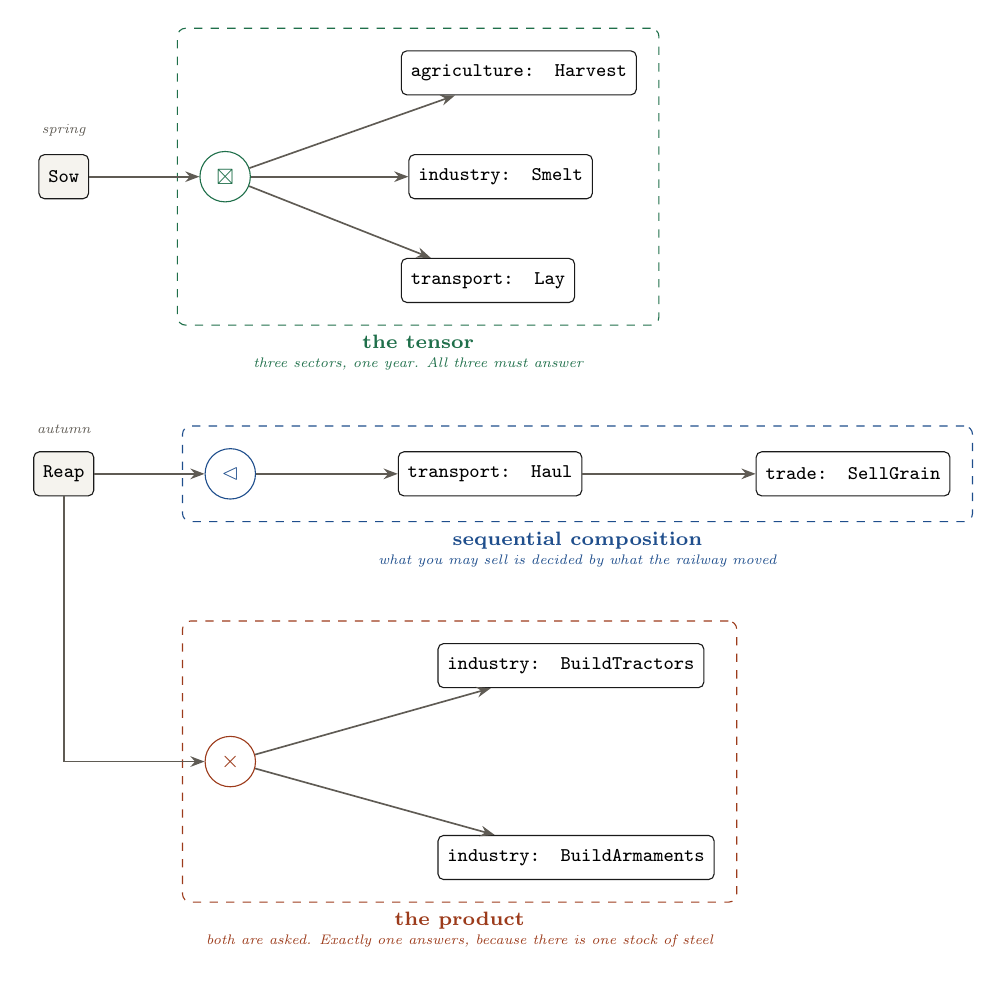
\begin{tikzpicture}

% --- SPRING: tensor ---
\node[plan] (sow) {Sow};
\node[lbl, above=1mm of sow] {spring};
\node[op, draw=tensor, text=tensor] (t1) [right=14mm of sow] {$\boxtimes$};
\node[srv] (agri)  [above right=8mm and 20mm of t1] {agriculture: Harvest};
\node[srv] (mill)  [right=20mm of t1]               {industry: Smelt};
\node[srv] (rail)  [below right=8mm and 20mm of t1] {transport: Lay};
\draw[ar] (sow) -- (t1);
\draw[ar] (t1) -- (agri);
\draw[ar] (t1) -- (mill);
\draw[ar] (t1) -- (rail);
\begin{scope}[on background layer]
\node[fit=(t1)(agri)(mill)(rail), draw=tensor, dashed, rounded corners=3pt,
      inner sep=2.8mm, label={[capt, text=tensor, align=center]below:%
      the tensor\\[-0.4mm]
      {\normalfont\itshape\tiny three sectors, one year. All three must answer}}] {};
\end{scope}

% --- AUTUMN: seq ---
\node[plan] (reap) [below=32mm of sow] {Reap};
\node[lbl, above=1mm of reap] {autumn};
\node[op, draw=seq, text=seq] (s1) [right=14mm of reap] {$\lhd$};
\node[srv] (rail2) [right=18mm of s1]    {transport: Haul};
\node[srv] (trade) [right=22mm of rail2] {trade: SellGrain};
\draw[ar] (reap) -- (s1);
\draw[ar] (s1) -- (rail2);
\draw[ar] (rail2) -- (trade);
\begin{scope}[on background layer]
\node[fit=(s1)(rail2)(trade), draw=seq, dashed, rounded corners=3pt,
      inner sep=2.8mm, label={[capt, text=seq, align=center]below:%
      sequential composition\\[-0.4mm]
      {\normalfont\itshape\tiny what you may sell is decided by what the railway moved}}] {};
\end{scope}

% --- PRODUCT ---
\node[op, draw=prod, text=prod] (p1) [below=30mm of s1] {$\times$};
\node[srv] (tract) [above right=7mm and 24mm of p1] {industry: BuildTractors};
\node[srv] (arms)  [below right=7mm and 24mm of p1] {industry: BuildArmaments};
\draw[ar] (reap) |- (p1);
\draw[ar] (p1) -- (tract);
\draw[ar] (p1) -- (arms);
\begin{scope}[on background layer]
\node[fit=(p1)(tract)(arms), draw=prod, dashed, rounded corners=3pt,
      inner sep=2.8mm, label={[capt, text=prod, align=center]below:%
      the product\\[-0.4mm]
      {\normalfont\itshape\tiny both are asked. Exactly one answers, because there is one stock of steel}}] {};
\end{scope}

\end{tikzpicture}
\end{center}

\vspace{6mm}

\section{The prompt}

I am an agentic engineer. I generate code using agentic coding agents such as Claude Code, Grok and
Codex. The following description is a rough approximation of the prompt I gave Claude to build the
game.

\begin{listbox}
\textbf{You want to build tractors.} The peasants are starving. More tractors means more grain, and
peasants can be moved off the land to work on railways and in steel mills.

\textbf{You need steel to build tractors.} You also need steel to build armaments. Steel needs a
mill. A mill needs a German engineer.
An engineer has to be paid in hard currency. Hard currency comes from selling grain to the USA.

\textbf{You need to build railways.} You cannot sell the grain without railways. Railways need steel too, but they are not capital. They are \emph{throughput}. Grain the railway cannot
move rots at the sidings, whatever the harvest was. So track comes before tonnage. This is the
sequential operator $\lhd$. What may be sold is computed from what the railway managed to move.

\textbf{You can buy tractors and steel.} But this will not mechanise the country.

\textbf{You must prepare for war.} In 1941 the country is invaded. Peasants serve as the soldiers, so the same population is both the workforce and
the army. Steel not spent on tractors or train tracks can be spent on armaments instead. Fight with too
little steel and you win by sending more men. Fight with more steel and send fewer peasants to die. Fail to arm at
all and no amount of mechanisation saves you.

\textbf{You must also feed the peasants.} The labour force is one pool of people. They can work the
fields, drive the tractors, work the mill or lay the track. But everyone eats, and only the first
two grow anything. That is why moving a peasant into the mill costs you twice.

\textbf{The Soviet Union is a centrally planned economy.} How hard the villages are squeezed is a decision
you make every spring. What is not taken is what
they eat. Starvation in this game is not a scoring gimmick. It is the direct arithmetic consequence
of the extraction and investment decisions made each spring and autumn, which is what it was for
Stalin.

\textbf{There are three goals.} Mechanise the country, win the war, and starve as few people as
possible.
\end{listbox}

To say that the game was generated by a single prompt would be a lie. But it is not far from the
truth. I pointed Claude at Ghani's note on containers for agentic AI, chatted to him a little bit
about CLI tools and TypeScript \texttt{async} functions, then gave him a somewhat vague description
of what I wanted the game to do, similar to the one above. He did the rest. What falls out is how
well suited Ghani's container combinator theory is for modelling this game.


\newpage

\section{Strategy}
\label{sec:strategy}

\begin{sectionbox}
The game has been built, by Claude Code, and is playable. Just pull the repo and type
\texttt{./play}.

\begin{center}
\texttt{github.com/RaggedR/stalin}
\end{center}

Try it out for yourself.
\end{sectionbox}

\textbf{A year is two turns, spring and autumn.} In spring you allocate labour and decide how hard
to squeeze the peasants. In autumn the harvest comes in graded, and you allocate it to tractors,
train tracks or armaments knowing exactly how much came in. Five years is ten decisions, and then
the war.

\textbf{Buy the tractors or build them yourself.} This is one of the first decisions that you must
make in the game.

\textbf{Build them.} Takes time. Hard currency buys a German engineer. The engineer raises the
mill. The mill makes steel. Twenty spare tonnes of steel opens the works. The works makes twenty
tractors a year forever. But you don't get your first tractor until 1930.

\textbf{Buy them.} Ten in hard currency each, ready to drive. They need no engineer, no mill and no
works. They build none of those either. You need to buy the tractor again each year.

\subsection{Seven plans}

It is a very simple game. Ten turns. At each turn you choose an option from the menu A-J.

\begin{center}\small
\begin{tabular}{@{}llrrrrrl@{}}
\toprule
strategy & letters & tractors & armaments & starved & fallen & \textbf{dead} & outcome \\
\midrule
bought tractors   & \texttt{AMAMAFAMAF} & 18 &  0 &  3 & 57 & \textbf{60} & \emph{lost} \\
never armed       & \texttt{CAKEBINIAI} & 62 &  0 & 15 & 52 & \textbf{67} & \emph{lost} \\
partial armament  & \texttt{CABEBINJAA} & 42 & 34 & 21 & 14 & \textbf{35} & won, mechanised \\
gentle armament   & \texttt{AJBEBJAJAJ} &  2 & 89 &  5 &  4 & \textbf{9}  & won \\
brutalist mech.   & \texttt{CMKEBIBJNJ} & 22 & 80 & 14 &  5 & \textbf{19} & won, mechanised \\
no railway        & \texttt{KABEBIBJAJ} & 22 & 82 & 25 &  4 & \textbf{29} & won, mechanised \\
totally brutal    & \texttt{KJBEAJBJAJ} &  2 & 78 & 44 &  5 & \textbf{49} & won \\
\bottomrule
\end{tabular}
\end{center}

\vspace{5mm}

\textbf{Never arming loses the war.} Sixty-two tractors. But no more Russia.

\textbf{Buying the tractors is humane but fatal.} Three starve, the fewest of any strategy. But
imported tractors build no mill, no engineers and no steel. So there is nothing to arm with, and
Russia is destroyed.

\textbf{Partial armament.} Mechanise first, build tractors, then arm. Less people starve, but you
have less steel for the war effort. More soldiers die.

\textbf{The railway should come before the steel.} Grain the railway cannot move rots before it can
be sold. Peasants starve. The total number of dead is still less for no railway than for partial
armament, because steel which would have been invested in the railway is invested in armaments.

\textbf{Total brutality.} Starving the peasants to build the army wins the war. But it also fails
to mechanise the country.

\subsection{A surprise}

The parameters of the game were tuned, by Claude Code, so that the \emph{brutalist mechanisation}
strategy would be optimal. Starve the villages
early. Spend it on rail, engineers and tractors. Then turn the surplus into an army. This was
Stalin's strategy. It is morally uncomfortable and it was supposed to win.

It does not. At least not in terms of total numbers dead. The gentle armament strategy wins with
only 9 dead by doing almost nothing. It was found by machine search over the menu rather than by
hand. Put hands in the mill. Buy one German engineer. Then smelt straight into armaments for four
years. No railway. No tractors on purpose. And no famine beyond the baseline five who die whatever
you do.

But with this strategy the country is still not mechanised at the end of the war. Only two
tractors.


\newpage

\section{The Unix operating system, pipes, and CLI tools}
\label{sec:unix}

In case you are a little rusty we review some basic ideas about the Unix operating system. This
might be useful to Neil. I found it useful to write it all down. If you are already familiar with
Unix then skip this section.

\subsection{A process}

A \emph{process} is one running program, together with everything the kernel keeps on its
behalf. Its memory. Its position in the code. Its identity -- meaning which user it runs as. And a
number.

A program is a file sitting on a disk, and does nothing. A process is that file in motion. Run the
same program twice and you have two processes. They share nothing and cannot see each other.

The number is the process's \emph{pid}. It is how anything outside the process refers to it, and
there is no other handle. To stop a program you send a signal to its pid.

Every process has a parent. The kernel is not a process. At boot it creates the first process, and
that first process launches all the others.

On my MacBook Air the first process is called \texttt{launchd}. On Linux it is \texttt{init} or
\texttt{systemd}. Its own parent is given as 0, which is not a real process.

\subsection{User space and kernel space}

A running machine is divided in two. Your code executes in \emph{user space}. There it may do
arithmetic, compare values, jump from one place in its own code to another, and read and write the
memory that belongs to it. That is the whole of what it may do. It cannot address a disk, a network
card, or another process's memory. The physical processor is in a mode that forbids it. The \emph{kernel} executes
in kernel space, where every device and every process's memory is addressable. The division is
enforced by the hardware, not by convention.

There is exactly one interface between the two. It is the \emph{system call}. It suspends your
process, switches the physical processor into kernel mode, runs kernel code on your process's behalf, and
returns. Every effect a program has on the world outside its own memory is a system call. There is
no other mechanism.

\subsection{\texttt{read} and \texttt{write}}

That interface could have been wide. It is in fact very narrow. The two calls that matter most
are these:

\begin{lstlisting}[language=SH]
read (n, buffer, count)   -- give me up to count bytes from the thing numbered n
write(n, buffer, count)   -- take these count bytes and put them in the thing numbered n
\end{lstlisting}

Each takes a number identifying something already open, a place to put bytes or take them from,
and how many. Between them they are very nearly the whole interface to the outside world. What that
number is, and where it comes from, is the subject of two subsections below.

\subsection{Everything is a file}

Why should two calls be enough? Because of a design decision usually stated as a slogan.
``Everything is a file.'' A file on a disk, a terminal, a network connection, a source of
random bytes. All of them are presented to user space through the same interface. So the same two
calls reach all of them.

The slogan overstates itself in one respect, and it is worth being precise about which. Things do
differ in how they are \emph{made}. A file is opened by name. A network connection has to be built
by a short sequence of calls of its own. What they do not differ in is how they are \emph{used}.
Once the thing exists and you are holding its number, \texttt{read} and \texttt{write} are the whole
vocabulary. The uniformity is at the point of use. That is the point that matters, because using is
where one program meets another.

\subsection{File descriptors}

That number is a \emph{file descriptor}. It is a small non-negative integer. It is an index into the
\emph{file descriptor table}, which the kernel keeps for each process, and whose entries point at
the things that process has open.
Nothing in the number says what kind of thing it is. The descriptor is an opaque handle. That is
exactly why one program can be pointed at a file one day and at a network connection the next
without being rewritten.

Three entries are filled in before a process begins, and it did not fill them in itself. Whoever
started it did.

\begin{lstlisting}[language=SH]
0   standard input    the stream the program reads
1   standard output   where its results go
2   standard error    where its complaints go
\end{lstlisting}

Start a program from a terminal and all three point at that terminal. That is why results and
complaints appear jumbled together in one scrolling window. It is a property of the terminal, not
of the program.

\subsection{\texttt{cat}}

Everything so far is enough to write a real Unix program. The program \texttt{cat} is named for
\emph{concatenate}. It copies its input to its output, unchanged, and does nothing else. That is
its entire specification. It is almost exactly \texttt{read} and \texttt{write} in a loop.

\begin{lstlisting}[language=SH]
char buf[4096];
for (;;) {
    n = read(0, buf, 4096);   -- take up to 4096 bytes from standard input
    if (n == 0) break;        -- 0 bytes means end of input; stop
    if (n <  0) exit(1);      -- negative means the read itself failed
    write(1, buf, n);         -- put exactly those n bytes on standard output
}
\end{lstlisting}

The real \texttt{cat} is longer. The extra length is all flags and error messages. That loop is
the program. Look at what it does \emph{not} contain. It never asks what \texttt{0} is attached to,
or what \texttt{1} is attached to, because \texttt{read} and \texttt{write} provide no way to ask.
A disk file, a keyboard, another program's output. The loop is identical and the program cannot
tell the difference.

\subsection{\texttt{fork} and \texttt{exec}}

Two more system calls, and they are the two that make new processes.

The call \texttt{fork} \emph{duplicates} the calling process. Where there was one process there are now
two. They are identical in their memory, their open descriptors and their position in the code.
They differ only in the pid \texttt{fork} handed back. That is how each tells whether it is the
original or the copy.

The call \texttt{exec} \emph{replaces} the program running inside a process. Same process, same pid, same
file descriptor table. But the old code and memory are discarded and a new program is loaded in their
place.

Neither is a ``run this program'' call, and that is the point. To start a program, a process
\texttt{fork}s, and then the copy \texttt{exec}s. The file descriptor table survives both, so the copy
inherits the original's descriptors. And in the gap between the two calls the copy is still running
the original's code, so it can rearrange its own table before replacing itself. Three subsections
below turn on that gap.

\subsection{The shell}

The shell is not part of the kernel and has no privilege you do not have. It is an ordinary
process running in user space with your identity, and its purpose is to start other processes. That
is all it is. A process whose job is starting other processes.

\subsubsection{The environment}

A process carries one more thing. Its \emph{environment} is a set of named strings held
alongside its memory and its file descriptor table. They are called variables, but they are only ever
text. Like the file descriptor table, the environment survives \texttt{fork} and \texttt{exec}. So a new
process starts with a copy of the one that started it.

\begin{lstlisting}[language=SH]
$ export GREETING=hello     -- add it to this shell environment
$ sh -c 'echo $GREETING'    -- a different process, started by this one
hello
\end{lstlisting}

That is the whole of it: named text, inherited downwards. The most used of them is
\texttt{PATH}, which holds a list of directories; the shell searches them whenever it is
looking for a program to run.

\subsubsection{Globbing}

A word containing \texttt{*}, \texttt{?} or \texttt{[\,\ldots]} is a \emph{glob}: a pattern to
be matched against the names of files that exist. The symbol \texttt{*} stands for any run of characters,
\texttt{?} for a single one, \texttt{[abc]} for one character out of a set.

The matching is done by the shell, before any program is started:

\begin{lstlisting}[language=SH]
$ echo *.txt
log.txt notes.txt other.txt
\end{lstlisting}

The command \texttt{echo} prints its arguments and nothing else. So what it printed is exactly what it was
given, namely three filenames. It never saw an asterisk. That is why every program accepts
patterns, and why no program contains any code for matching them.

\subsubsection{What the shell does with a line}

Given a line, the shell does five things, and every one of them has already been described.

\begin{enumerate}
\item \textbf{Split the line into words.} The first word names what to run. The rest become the
      argument vector that program will receive.
\item \textbf{Find the program.} The first word is looked for in each directory named by
      \texttt{PATH}, in order, and the first match wins.
\item \textbf{\texttt{fork}.} The shell duplicates itself.
\item \textbf{\texttt{exec}.} The copy replaces itself with the program. The shell that read
      the line is still there, waiting for it to finish.
\item \textbf{Keep the exit status.} When the program finishes the kernel gives the shell a
      small number it left behind, by convention zero for success.
\end{enumerate}

One command cannot work that way, and the reason is worth seeing. The command \texttt{cd} has to be built
into the shell rather than being a program. A program runs in the copy, and the copy changing its
own working directory would leave the shell exactly where it was. Anything that must alter the
shell's own state has to be part of the shell.

A remark, because this is the mechanism behind something that catches people out with coding
agents. Claude Code runs each shell command exactly as the shell runs a program. It forks, and the
copy execs. A \texttt{cd} in that command changes the copy's working directory, and the copy then
exits. So no command the agent runs can change the agent's working directory. The directory it was
launched in is the directory it has for the whole session. That is why you must start it in the project you
actually mean to work on.

\subsection{Redirection}

Now the gap between \texttt{fork} and \texttt{exec}. Writing \texttt{> log} after a command tells
the shell to do one thing in the copy, before exec'ing. Open the file \texttt{log} and put it in
slot~1.

\begin{lstlisting}[language=SH]
$ echo hello > log      -- slot 1 is now the file, not the terminal
$ cat log
hello
\end{lstlisting}

Writing \texttt{2> errs} redirects descriptor~2 in the same way. Nothing was added to \texttt{echo} to
make this work. The command \texttt{echo} cannot discover that it happened. It wrote to descriptor~1 exactly as
it always does. Redirection is the shell's syntax and the shell's doing, from beginning to end.

\subsection{Pipes}

A \emph{pipe} is a buffer the kernel will hand out on request. It comes with two descriptors.
One to write into, one to read out of. The symbol \texttt{|} is the same redirection as \texttt{>}, with a pipe
where the file was. The shell asks for a pipe, forks twice, puts the writing end in the left
program's slot~1 and the reading end in the right program's slot~0, and execs both.

\begin{lstlisting}[language=SH]
$ cat notes.txt | wc -l
       3
\end{lstlisting}

The command \texttt{wc -l} counts the lines on its standard input. It was given no filename and does not
know one exists.

Both programs run at the same time. The program \texttt{wc} does not wait for \texttt{cat} to
finish. The
buffer is finite, at $64 \times 1024$ bytes on Linux, and the kernel makes each side wait for the
other rather than growing it. When it is full, \texttt{cat}'s next \texttt{write} does not return
until \texttt{wc} has consumed something. When it is empty, \texttt{wc}'s next \texttt{read} does
not return until \texttt{cat} has produced something. Neither program contains a line of code about
this.

Two things follow, and both are worth having in mind.

A pipeline over a very large file needs no more memory than a pipeline over a small one. At no
moment does either process hold more than the buffer.

And the second program starts answering immediately rather than at the end. Take
\texttt{cat huge.log | grep x}. The command \texttt{grep} is handed the first $64 \times 1024$
bytes as soon as \texttt{cat} has written them, and reports its first match from those, while
\texttt{cat} is still reading. It does not need to wait for \texttt{cat} to finish. Nothing in
either program arranges for it not to. That is simply what two processes and one finite buffer
do.

\subsection{Threads}
\label{sec:threads}

The pipe in the previous subsection contained a piece of concurrency and did not draw attention to
it. The programs \texttt{cat} and \texttt{wc} run at the same time. It is worth asking what that
sentence can possibly mean. For this we need to understand threads.

\textbf{The physical processor is handed out in slices.}

Assume the machine has one physical processor. It executes one instruction stream. It has no notion
of a process. To run many processes on it the kernel keeps a set of flows of control it considers
\emph{runnable}, and gives the physical processor to one of them. A hardware timer interrupts a few milliseconds later. The kernel saves
that flow's registers and its position in the code, loads another's, and returns. The interrupted
process is not asked and cannot tell.

That is \emph{preemption}. The consequence to carry forward is a single sentence. A program's text
does not mark the points at which it may be interrupted, because every point between two machine
instructions is one.

\textbf{Blocking is the other way to lose the physical processor.}

When \texttt{wc}'s \texttt{read} finds the buffer empty, the kernel marks it \emph{not runnable}
and gives the physical processor to somebody else.

A blocked process consumes nothing at all. It
is not a candidate for scheduling until the thing it waits on becomes ready. Then the kernel makes
it runnable again and it resumes inside \texttt{read}, as though that call had merely been slow.

This is the default behaviour of nearly every system call that touches the world. It is why the
programs in the previous subsections could be written as straight lines, with no mention of waiting
anywhere in them.

\textbf{What the kernel keeps on a process's behalf.}

The bookkeeping falls into two lists, and the difference between them is what this section is
about.

The first list is what the process \emph{owns}. Its address space, meaning the tables that map the
addresses appearing in its code to real memory. Its file descriptor table. Its identity -- meaning
which user it runs as. Its pid.

The second list is what the kernel needs in order to \emph{run} it. Its position in the code, its
registers, and its stack.

Only the second list is required to give a process a slice of physical processor.

The first is what makes a
process expensive. Creating one means building page tables. Switching from one to another means the
physical processor's address-translation caches now describe the wrong process and must be refilled. The
first list is also what isolates. Two processes cannot see each other because neither address space
contains a mapping to the other.

\textbf{A thread is the second list on its own.}

A \emph{thread} is a flow of control. A position in the code, a set of registers, and a stack.
Nothing else. Every process begins with exactly one thread, and may ask the kernel for more.
Threads belonging to the same process share every item on the first list. They share one address
space, so every variable one of them can reach, all of them can reach. They share one file
descriptor table, so anything one of them opens is open for all of them. They share one identity
and one pid. What they do not share is the second list. Each has its own position in the code, its
own registers, and its own stack.

The kernel schedules threads, not processes. Blocking is therefore per-thread. One thread stuck
inside \texttt{read} leaves its siblings runnable, and that is the whole reason to want more than
one.

Threads are much cheaper than processes. All they need is their own stack, and a stack is
typically only a few megabytes of reserved address space.


\subsection{Exit status, and the shell's control flow}

The small number a program leaves behind is what the shell builds its control flow on.

\begin{itemize}
\item \texttt{;} \ \ run the next command regardless of the status.
\item \texttt{\&\&} \ \ run the next command only if the previous one exited zero.
\item \texttt{||} \ \ run the next command only if the previous one exited non-zero.
\item \texttt{\&} \ \ start this command and do not wait for it, so several can run at once.
\end{itemize}

We could say a good deal more about all this. It is not really relevant to the game
\texttt{stalin}.

\subsection{Shell scripts}

A file of such lines is a shell script, and running it is the same as having typed them. So a
pipeline that worked once can be kept and named. And a script is started like any other program. It
is found on \texttt{PATH}, \texttt{fork}ed, \texttt{exec}ed, and its status collected. So a script
can appear in a pipeline itself, on either side, and nothing that uses it needs to know it is a
script.

\subsection{Three channels, not one}

Gather up what a program actually offers the world outside it. There are three separate
channels, and they carry three different kinds of thing.

\begin{center}
\begin{tabular}{lll}
\toprule
\textbf{Channel} & \textbf{Carries} & \textbf{Read by} \\
\midrule
descriptor 1 (stdout) & the results  & the next program in the pipeline \\
descriptor 2 (stderr) & the narration & a person \\
the exit status       & the verdict  & the shell \\
\bottomrule
\end{tabular}
\end{center}

Keeping them apart is what makes a program usable by another program. A pipe takes descriptor~1
and nothing else. So whatever reads from a program receives its results, and never has to sort them
out from error text. Putting results and narration both on descriptor~1 is the commonest way to
make a program unusable in a pipeline.

\subsection{Manual pages, and what is not checked}

None of the above is checked by anything. The interface between two programs is bytes. Any two
can be joined. That is the strength. Nothing verifies that the composition means anything. That is
the cost. What a program promises is written in its manual page and nowhere else. So the only thing
enforcing it is that you read it.

This is a deliberate design choice.

\subsection{The Unix philosophy}

Let's summarise what we have. One uniform interface reached by \texttt{read} and \texttt{write}.
Three separate channels. A pipe that joins one program to another. With that on the table, the Unix
philosophy reads as a consequence of the machinery rather than as an aspiration. Doug McIlroy wrote
the pipe into Unix v3 in 1973. He put it in three sentences.

\begin{quote}
Write programs that do one thing and do it well. Write programs to work together. Write
programs to handle text streams, because that is a universal interface.
\end{quote}

Mike Gancarz later expanded this into nine tenets. Small is beautiful. Each program does one
thing well. Build a prototype as soon as you can. Choose portability over efficiency. Store data in
flat text. Use software leverage. Use scripts to increase leverage and portability. Avoid captive
user interfaces. Make every program a filter.

The last is the one that matters here, and it is the least obeyed. A \emph{filter} is a program
that reads a stream and writes a stream. Its input is not a dialogue. Its output is not a report to
a human. The programs \texttt{cat}, \texttt{wc} and \texttt{grep} are filters. That is why the examples above
could be assembled without any of them having been designed for each other.

\newpage

\section{CLI tools}
\label{sec:cli}

\begin{sectionbox}
A CLI tool is already a container.

A command-line tool receives one prompt, its argument vector. It produces a response whose
\emph{type depends on which prompt it was}.

For example the command \texttt{git log} answers with a list of commits. The command
\texttt{git status} answers with a working tree. Those are not the same kind of thing, and which
kind you get is fixed by the word after \texttt{git}.

The interface is documented in the man pages. But there is \emph{no type checker}. Nothing verifies
whether the output from one CLI tool piped into the input of another has the right type.

It is up to the developer to check that the interfaces match.

A professional in formal verification would find this claim horrifying. If there is no type
checker then what does it mean to have a type? Well, Python has no type checker. It doesn't mean
it has no types. It just means we don't check them.

More importantly, the Claude Code harness is a CLI tool, and it prints its response to the
standard output. We are more interested in how it delegates its prompt to the other CLI tools
that it calls than in the response to that prompt.

\label{sec:harness}

The Claude Code harness is itself just another CLI tool. This is worth stopping and reflecting
upon. It is what makes this design so beautiful.

You run it with a prompt as its argument, and it answers on standard output.

\begin{lstlisting}[language=SH]
$ claude -p 'Reply with exactly the four words: this is a reply'
this is a reply
\end{lstlisting}

The Claude Code harness is a CLI tool that executes other CLI tools. When it runs a command it does
what the shell does. It \texttt{fork}s. The copy \texttt{exec}s. The copy inherits its parent's identity.

That's it. It runs with the permissions of the user that executed it. It can read and write any
file that user can read and write, and it can execute any command that user can execute.

The Claude Code harness also calls other CLI tools. That is nearly the whole of what it does. It
reads a prompt, decides which commands to run, forks and execs them, reads what they wrote, and
replies.

You can set him up with limited privileges, a handful of CLI tools that he has permission to
operate and nothing else.
\end{sectionbox}

\newpage

\section{HTTP and JSON}
\label{sec:http}

We don't assume that you know anything about web app development, so we review here the basics of
the HTTP protocol and the JSON datatype.

The simplest kind of web app runs a database on a server. The client, a CLI tool, sends a HTTP
request across the wire to a server. The server usually runs on a separate machine from the
client, but in our case it will run on the same machine.

If it is a read request, then the server reads from a database and either returns the result
across the wire as a second HTTP request or it returns an error. If it is a write request,
then the server takes the body of the HTTP request as instructions for what to write to the
database, and returns either success or an error.

You don't need to know what a database is, except on the most intuitive level. Claude will happily
write you a simple web app of this form without you even needing to know anything about HTTP or
JSON.

The examples below all run against a toy server whose database is a list of books. It has nothing
to do with the game, which does not have a database. It exists to introduce HTTP and JSON.

\subsection{A request and a response}

HTTP is a request/response protocol. A client sends a request. A server sends a response. Nothing
else happens. Here is one complete exchange, the request and the response.

\begin{center}
\colorbox{codebg}{\begin{minipage}{0.95\linewidth}\ttfamily\small
\setlength{\fboxsep}{1.5pt}\vspace{1mm}
\mbox{> GET /books/13 \colorbox{linebg}{HTTP/1.1}}\\
\hspace*{1em}\colorbox{hdrbg}{\mbox{Host: 127.0.0.1:8099}}\\
\hspace*{1em}\colorbox{hdrbg}{\mbox{Accept: */*}}\\
\mbox{}\\
\mbox{< \colorbox{linebg}{HTTP/1.1} 200 OK}\\
\hspace*{1em}\colorbox{hdrbg}{\mbox{Content-Type: application/json}}\\
\hspace*{1em}\colorbox{hdrbg}{\mbox{Content-Length: 53}}\\
\mbox{}\\
\hspace*{1em}\colorbox{bdybg}{\mbox{\{"id": 13, "title": "Diaspora", "author": "Greg Egan"\}}}
\vspace{1mm}
\end{minipage}}
\end{center}

That's it. A request is a \emph{method} (\texttt{GET}), a \emph{path} (\texttt{/books/13}), some
\emph{headers} (blue), and optionally a \emph{body} (none in this example). A response is a
three-digit \emph{status} (\texttt{200}), some headers (blue), and a body (green).

\subsection{Deliberately simple}

The designer of the HTTP protocol, Roy Fielding, made the same kind of design decision that Unix
made. And it paid off. Just as every server in the world today runs Unix, every web app in the
world today communicates via HTTP.

\newpage

\subsection{The method says what kind of thing you are doing}

There are four types of HTTP request. We only use two of them.

\begin{center}
\begin{tabular}{ll}
\toprule
\textbf{Method} & \textbf{Means} \\
\midrule
\texttt{GET}    & read something, change nothing \\
\texttt{POST}   & create something \\
\bottomrule
\end{tabular}
\end{center}

As we already mentioned, a simple web app runs a database on the server. When the server receives
a \texttt{GET} request it reads the database and returns the result to the client, or returns an
error. When the server receives a \texttt{POST} request it either writes to the database or returns
an error.

In our ``toy example'' the database simply contains a collection of books with their title and
author. Each book has a unique ID number.

Here is an example of reading the book with ID 13 from the database.

\begin{lstlisting}[language=SH]
$ curl -X GET http://127.0.0.1:8099/books/13
{"id": 13, "title": "Diaspora", "author": "Greg Egan"}          -- 200 OK
\end{lstlisting}

It is worth breaking down the address of a single book.

\begin{center}
\colorbox{codebg}{\begin{minipage}{0.95\linewidth}\centering\ttfamily\small
\setlength{\fboxsep}{1.5pt}\vspace{1.6mm}
\mbox{\colorbox{linebg}{http}://\colorbox{hdrbg}{127.0.0.1}:\colorbox{bdybg}{8099}\colorbox{pathbg}{/books/13}}
\vspace{1.6mm}
\end{minipage}}
\end{center}

\begin{center}\small
\begin{tabular}{@{}ll@{}}
\toprule
\textbf{Part} & \textbf{Meaning} \\
\midrule
\colorbox{linebg}{\texttt{http}}      & the protocol to speak \\
\colorbox{hdrbg}{\texttt{127.0.0.1}}  & the machine, which here is this one, known as \emph{localhost} \\
\colorbox{bdybg}{\texttt{8099}}       & the port, which says which program on that machine \\
\colorbox{pathbg}{\texttt{/books/13}} & the path, which says which thing that program should answer about \\
\bottomrule
\end{tabular}
\end{center}

The command \texttt{curl} is just another Unix CLI tool. It sends one HTTP request across the wire
and prints the response to the standard output.

Note that since ``everything is a file'' the Unix kernel handles all the networking, and
\texttt{curl} just thinks it is reading to and writing from a file.

We say that the server is ``listening'' on port 8099. What this really means is that the kernel
has created a socket with unique ID number 8099 and handed it as a unique file descriptor to the
server. The kernel handles all the networking and the server thinks it is reading and writing to
a file. So we can forget about ``the wire''.

This is essentially the same as a Unix pipe, only instead of communicating via plain text we are
communicating via HTTP with JSON bodies -- which is a form of structured text.

Here is an example of adding a new book to the database.

\begin{lstlisting}[language=SH]
$ curl -X POST http://127.0.0.1:8099/books \
       -H 'Content-Type: application/json' \
       -d '{"title":"Anna Karenina","author":"Leo Tolstoy"}'
{"id": 27, "title": "Anna Karenina", "author": "Leo Tolstoy"}   -- 201 Created
\end{lstlisting}

\subsection{JSON}

JSON is short for JavaScript Object Notation. It is a recursive text format for data. Just like
HTTP it is deliberately simple. It has four types of ``atomic'' data: numbers, strings, booleans
and \texttt{null}. Then it has two recursive constructors: array and object.

\begin{lstlisting}
value  ::=  string | number | boolean | null
         |  '[' value* ']'
         |  '{' (string ':' value)* '}'
\end{lstlisting}

To keep things even more simple, we will assume that the bodies of our requests and responses are
well formed JSON. This is not so simple if you are interested in formal verification but that is
not our focus here.

\newpage

\section{TypeScript}
\label{sec:respval}

In our case the server is written in TypeScript. TypeScript is an interpreted language, and the
CLI tool \texttt{deno} is the interpreter.

We do not have a database. Instead the server calls local CLI tools, amalgamates the responses,
and either returns the result or returns an error. The result gets ``piped back'' to the client
via HTTP and JSON. Both the client and the server are running on the same machine.

Inside a TypeScript program the two halves of the exchange between the client and the server are
ordinary values, and they have names. A \texttt{Request} is one arriving HTTP request. A
\texttt{Response} is one outgoing HTTP response.

\begin{sectionbox}
We don't assume that you know TypeScript. I don't know TypeScript. Claude knows TypeScript.
The companion note \emph{TypeScript Syntax} is a ``crash course'' on TypeScript syntax and the
somewhat bizarre TypeScript type system.
\end{sectionbox}

A \texttt{Response} inside TypeScript is built from the three things extracted from the HTTP
response. A body, a status number, and a set of headers.

\begin{lstlisting}[language=TS]
const body = JSON.stringify({ id: 13 });

const res = new Response(body, {
  status: 200,
  headers: { "content-type": "application/json" },
});

console.log("body   :", body);
console.log("status :", res.status);
console.log("header :", res.headers.get("content-type"));
\end{lstlisting}

This should be relatively self-explanatory. The body is a string.

Save this in the file \texttt{r.ts}. Now in the terminal.

\begin{lstlisting}[language=SH]
$ deno run r.ts
body   : {"id":13}
status : 200
header : application/json
\end{lstlisting}

A server handler is a function that returns a \texttt{Response}.

The body of a \texttt{Request} arrives on a socket, which, as we already mentioned, just looks
like a file to the \texttt{deno} server. Getting it requires a system call \texttt{read}, and as
discussed in Section~\ref{sec:threads} a system call can block.

Threads are not the solution here. A server may hold multiple conversations while only one of
them is doing anything. One client may be adding the book \emph{The Picture of Dorian Gray} while
a second is adding the book \emph{Visual Complex Analysis}. Adding a book to the database is
really a system call to \texttt{read} followed by a system call to \texttt{write}. These can
accidentally become interleaved.

\newpage

The server keeps track of the next available ID number for a new book to be added in a variable
on the server.

Suppose the next available ID for a new book is 40, and two clients add a book at once. Both
threads read 40. Both give 40 to their book. Both write 41 as the next available ID number. Two
books now have ID 40. This is a problem.

Section~\ref{sec:async} is about what the server does to solve this problem. And it is the
mechanism by which we ``fake'' containers.

\newpage

\section{\texttt{async}, \texttt{await}, and the event loop}
\label{sec:async}

\begin{sectionbox}
The \texttt{deno} interpreter provides a small web server. The web server owns the event loop.
This is how we ``fake'' containers.
\end{sectionbox}

\subsection{One flow of control, and it may not stop}
\label{sec:oneflow}

A server holds many conversations at once, most of them idle most of the time. If we are running a
proper library then hundreds or thousands of people could be borrowing and returning books. A
single flow of control can only serve one of them at a time.

The design used by \texttt{deno} keeps one flow of control and never lets it block. Every operation
that would have waited is written in three parts instead.

\begin{enumerate}\setlength{\itemsep}{2pt}
\item \textbf{Start it.} Ask for the thing, and do not wait for it.
\item \textbf{Give the flow of control back.} Stop, so that the other conversations can be served.
\item \textbf{Arrange to be resumed.} Leave behind what should happen when the response arrives.
\end{enumerate}

Something has to hold those arrangements. That something is the \textbf{event loop}. It is a set of
outstanding resumptions, each of them waiting on one thing, together with a way of asking which of
those things are ready now. The loop takes one that is ready, runs it, and asks again for the next
one. It never blocks on any particular conversation because it never commits to one.

\subsection{Inversion of control}

This arrangement is called \emph{inversion of control}.

\begin{orestisbox}
The type \texttt{Promise<T>} is a computation of a \texttt{T} that has not finished yet.
\end{orestisbox}

Composition is where the difference shows. Write $g \circ f$ for ``apply $f$, then $g$''. In an
ordinary program the two functions join up and the type is the one you expect.

\begin{center}\small
\begin{tabular}{@{}ll@{}}
\toprule
$f$          & \texttt{<T, R>(x: T) => R} \\
$g$          & \texttt{<R, S>(y: R) => S} \\
$g \circ f$  & \texttt{<T, S>(x: T) => S} \\
\bottomrule
\end{tabular}
\end{center}

In the event loop neither function can return its answer, because neither answer exists yet. Each
returns a promise of one instead.

\begin{center}\small
\begin{tabular}{@{}ll@{}}
\toprule
$f$          & \texttt{<T, R>(x: T) => Promise<R>} \\
$g$          & \texttt{<R, S>(y: R) => Promise<S>} \\
$g \circ f$  & \texttt{<T, S>(x: T) => Promise<S>} \\
\bottomrule
\end{tabular}
\end{center}

The types can no longer be composed. The first function $f$ returns an output of type
\texttt{Promise<R>} but the second function $g$ expects an input of type \texttt{R}.

\newpage

\begin{sectionbox}
The type constructor \texttt{Promise} \emph{looks like} a monad, and it \emph{looks like} what is
needed is \emph{some sort} of \emph{Kleisli composition}. It is not actually a monad, and if you
feel like torturing yourself you can check that it doesn't satisfy the monad laws. But you can
still think of it in terms of unit and bind.

The keyword \texttt{async} is the unit, taking a value to a promise already holding it. The
keyword \texttt{await} is the bind, taking a promise and a function from its value to a second
promise.

The keyword \texttt{await} unwraps the \texttt{Promise<R>} so that $g$ may be applied to it. The
keyword \texttt{async} wraps the answer back up. Everything between them is ordinary
composition.
\end{sectionbox}

The composition function we are looking for is the following.

\begin{lstlisting}[language=TS]
const compose =
  <T, R, S>(f: (x: T) => Promise<R>, g: (y: R) => Promise<S>) =>
  async (x: T): Promise<S> => g(await f(x));
\end{lstlisting}

The call \texttt{Promise.resolve(x)} builds a promise that has already finished, holding
\texttt{x}. We give an example below.

\begin{lstlisting}[language=TS]
const parse  = (s: string): Promise<number> => Promise.resolve(s.length);
const render = (n: number): Promise<string> => Promise.resolve("#".repeat(n));

const both: (x: string) => Promise<string> = compose(parse, render);
console.log(await both("secret"));
\end{lstlisting}

The function \texttt{both} could be used to hide a password, for example. Now run it in the
terminal:

\begin{lstlisting}[language=SH]
$ deno check compose.ts
$ deno run compose.ts
######
\end{lstlisting}

\newpage

Let's add logging now to see what order things happen in. First, composition of normal functions.

\begin{lstlisting}[language=TS,
  linebackgroundcolor={\ifnum\value{lstnumber}=4\color{hdrbg}\fi
                       \ifnum\value{lstnumber}=6\color{hdrbg}\fi}]
const compose_normal =
  <T, R, S>(f: (x: T) => R, g: (y: R) => S) =>
  (x: T): S => {
    console.log("part 1");
    const r = f(x);
    console.log("part 2");
    return g(r);
  };

const f_normal = (s: string): number => s.length;
const g_normal = (n: number): string => "#".repeat(n);
const both_normal = compose_normal(f_normal, g_normal);
const b = both_normal("secret");
console.log("both_normal has returned");
console.log(b);
\end{lstlisting}

Save this to the file \texttt{normal.ts} and run it in the terminal:

\begin{lstlisting}[language=SH]
$ deno run normal.ts
part 1
part 2
both_normal has returned
######
\end{lstlisting}

Both parts run, and only then does the \texttt{compose\_normal} function return. This is the
normal order of control flow.

\newpage

Next, async composition:

\begin{lstlisting}[language=TS,
  linebackgroundcolor={\ifnum\value{lstnumber}=4\color{hdrbg}\fi
                       \ifnum\value{lstnumber}=6\color{hdrbg}\fi}]
const compose_log =
  <T, R, S>(f: (x: T) => Promise<R>, g: (y: R) => Promise<S>) =>
  async (x: T): Promise<S> => {
    console.log("part 1");
    const r = await f(x);
    console.log("part 2");
    return g(r);
  };

const parse_slow  = (s: string): Promise<number> =>
  new Promise((ok) => setTimeout(() => ok(s.length), 100));
const render_slow = (n: number): Promise<string> =>
  new Promise((ok) => setTimeout(() => ok("#".repeat(n)), 100));
const both_log = compose_log(parse_slow, render_slow);
const a = both_log("secret");
console.log("both_log has returned");
console.log(await a);
\end{lstlisting}

Here we have used a lambda function to make sure the functions $f$ and $g$ take some non-trivial
amount of time to return. Save the above to the file \texttt{why.ts} and then run it in the
terminal:

\begin{lstlisting}[language=SH]
$ deno run why.ts
part 1
both_log has returned
part 2
######
\end{lstlisting}

Note the order.

This is why we call it inversion of control. You do not call the second function. You give it
away.

\subsection{Async hell}
\label{sec:asynchell}

\begin{sectionbox}
Functions which depend on other functions which in turn depend on other functions form a tree.
Depending on how long each function takes to complete, they may return in any order which is a
linear extension of that tree.

For a complex dependency tree, writing out all the \texttt{async} and \texttt{await} keywords to
record the nesting structure is a nightmare. It is commonly referred to as \emph{async hell}.
This is exactly the problem that Ghani's container formalism solves.

The tree is a dependency order, which is a partial order. The event loop produces some
topological sort of it, and which one you get is decided by whichever promise settles first.

That is the gap the four combinators close. The tensor $\boxtimes$ says that two subtrees are
independent and may interleave. The sequential $\lhd$ says that one must precede the other. The
combinators are a language for writing down the partial order, so you no longer have to
hand-schedule a linear one.
\end{sectionbox}

\subsection{How it actually works}

You hand the loop a function called a \emph{handler}, and it calls that function once for each
request that arrives. Here is a whole server.

\begin{orestisbox}
A reminder from \S\ref{sec:respval}. A \texttt{Request} is one arriving HTTP request and a
\texttt{Response} is one outgoing HTTP response. A \texttt{Response} is built from a body, a status
number and a set of headers. A handler is a function from the first to the second. And we are
assuming throughout that the bodies of our requests and responses are well formed JSON.
\end{orestisbox}

\begin{lstlisting}[language=TS]
const json = (body: unknown, status: number) =>
  new Response(JSON.stringify(body), {
    status,
    headers: { "content-type": "application/json" },
  });

const census = async () => ({ fields: 30, drivers: 22, dead: 11 });

Deno.serve({ port: 8099 }, async (req) => {
  const body = await req.json();
  if (body.tag !== "Census") return json({ error: "not a prompt I accept", got: body }, 400);
  return json(await census(), 200);
});
\end{lstlisting}

Three lines of that are the handler. The rest builds a response.

Now send it a prompt it accepts, and then one it does not.

\begin{lstlisting}[language=SH]
$ curl -si -X POST http://127.0.0.1:8099/ -d '{"tag":"Census"}'
HTTP/1.1 200 OK
content-type: application/json

{"fields":30,"drivers":22,"dead":11}

$ curl -si -X POST http://127.0.0.1:8099/ -d '{"tag":"Nonsense"}'
HTTP/1.1 400 Bad Request
content-type: application/json

{"error":"not a prompt I accept","got":{"tag":"Nonsense"}}
\end{lstlisting}

Two things in that handler matter for everything below. The response is computed from the prompt, so
what comes back depends on what went in. And the function stops twice before it answers, once for
the request body and once for the response, which is the reason a loop has to exist at all.

\newpage

\begin{pinkbox}
\section{Conditional types}
\label{sec:cond}

Everything this note does depends on one construct, so it is worth going slowly.

A \emph{conditional type} is a function from types to types. It is a type constructor. It is
written with the same punctuation as an ordinary conditional expression, but it lives one level
up, and the checker evaluates it before the program runs.

Stay with the shelf of books. A book has three fields, and their names are \texttt{id},
\texttt{title} and \texttt{author}. Those three names form a finite union.

\begin{lstlisting}[language=TS]
type Field = "id" | "title" | "author";
\end{lstlisting}

\subsection{A function from types to types}

Now notice that the three fields do not hold the same kind of thing. An \texttt{id} is a number.
A \texttt{title} and an \texttt{author} are strings. That fact can be written down as a function,
on the level of types.

\begin{lstlisting}[language=TS]
type FieldType<F extends Field> =
  F extends "id" ? number : string;
\end{lstlisting}

The word \texttt{extends} appears twice there. Both times it means the same thing, namely
\emph{is a subtype of}. What differs is what is done with the answer.

In \texttt{<F extends Field>} it is a \emph{requirement}. The type \texttt{F} must be a subtype of
\texttt{Field}, which here means one of \texttt{id}, \texttt{title} or \texttt{author}. It ranges
over the field names, which are the keys of the dictionary. It does not range over the types of the
values stored under those keys.

In \texttt{F extends "id" ?} it is a \emph{question}. Is \texttt{F} a subtype of \texttt{"id"}?
That type has exactly one inhabitant, so the question amounts to asking whether \texttt{F} is
\texttt{"id"} itself. The answer selects one of the two branches. If \texttt{F} is not
\texttt{"id"} then it must be \texttt{"title"} or \texttt{"author"}. The value stored under either
of those keys is a string, so the second branch gives \texttt{string}.

\begin{orestisbox}
\subsection{Question for Orestis}

Is there anything equivalent to this in Haskell or Lean?
\end{orestisbox}

\newpage

\subsection{A function on the level of values}

The result type of the function below is computed from its argument type. It looks a little bit
like a dependent type, but that is not quite what it is.

\begin{lstlisting}[language=TS]
function field<F extends Field>(b: Book, f: F): FieldType<F> {
  return b[f] as FieldType<F>;
}

const n = field(book, "id");      // n : number
const s = field(book, "title");   // s : string
\end{lstlisting}

That is the whole trick. The type checker read the string \texttt{"id"}. It computed the type
\texttt{FieldType<"id">}. It concluded that \texttt{n} is a number. Knowing that is what tells the
checker which operations on \texttt{n} are legal.

\subsection{The fake container}

Compare this with the introduction. An interface was a pair there. The prompts you may send, and
for each prompt the type of response it can receive.

Here \texttt{Field} is the type of the prompts, and \texttt{FieldType} is the type of the response
for each prompt. So \texttt{(Field, FieldType)} is a container, and \texttt{field} is an inhabitant
of it.

\subsection{Two limits}

\begin{orestisbox}
\begin{itemize}\setlength{\itemsep}{4pt}

\item \textbf{The index must be finite.} \texttt{Field} has three members, so \texttt{FieldType}
      can be written out as a case split, here a single test and a default. Over a finite index a
      dependent type is just a table, and a table is something TypeScript can write down. A rule
      indexed by the natural numbers could not be written this way at all.

\item \textbf{The argument must be a literal the checker can see.} In
      \texttt{field(book, "id")} the string \texttt{"id"} is written in the source. So the checker
      infers \texttt{F} to be the singleton type \texttt{"id"}, and \texttt{FieldType<"id">}
      computes to \texttt{number}.

\end{itemize}
\end{orestisbox}

This is not as big a problem as it might seem. The field name does not have to be written in the
source. It can be typed at the terminal, which is the case that matters here, because a CLI tool
receives its prompt as an argument vector.

\begin{lstlisting}[language=TS]
const name = Deno.args[0] as Field;   // typed at the terminal, not in the source
const m = field(book, name);
const u: number = m;
\end{lstlisting}

What is the type of \texttt{m}?

\begin{lstlisting}[language=TS]
FieldType<"id">      is  number
FieldType<"title">   is  string
FieldType<"author">  is  string
\end{lstlisting}

Put those three answers together and \texttt{m} could be a number or it could be a string. So
\texttt{m} is of type \texttt{string | number}.

Why is this a problem? Because a name arrives at run time and you want to assign it to a
variable. The checker must be able to pin it to one member of the union. Testing the name does
exactly that, and inside each branch the dependency works again.

\begin{lstlisting}[language=TS]
const name = Deno.args[0] as Field;
if (name === "id") {
  const u: number = field(book, name);
  console.log("a number:", u);
} else {
  const u: string = field(book, name);
  console.log("a string:", u);
}
\end{lstlisting}

So it is not really a problem after all.

\subsection{Recovering the name}

To get it back you write a \texttt{switch} with one branch per name. Inside \texttt{case "id":} the
checker knows the name is \texttt{"id"} again, so \texttt{FieldType<"id">} is \texttt{number} once
more. It's a bit ugly but it works.

\end{pinkbox}

\newpage

\begin{pinkbox}
\section{Mapped types, which make a table total}
\label{sec:mapped}

The second construct to go slowly over is the one that builds a record with a field for every
member of a union.

Keep the same three field names.

\begin{lstlisting}[language=TS]
type Field = "id" | "title" | "author";
\end{lstlisting}

Suppose we want, for each field, a function that reads that field out of a book. There should be
exactly three of them, and each should return the right kind of thing. A mapped type says so.

\begin{lstlisting}[language=TS]
type Getters = { [F in Field]: (b: Book) => FieldType<F> };
\end{lstlisting}

Read \texttt{[F in Field]} as ``for every \texttt{F} in \texttt{Field}''. It generates one field
per member, and the field's type may mention \texttt{F}. So \texttt{Getters} is a record with three
fields, and their types are not the same as each other.

\begin{lstlisting}[language=TS]
const getters: Getters = {
  id:     (b) => b.id,        // must return number
  title:  (b) => b.title,     // must return string
  author: (b) => b.author,    // must return string
};
\end{lstlisting}

That version compiles. Now the point of the whole thing. The record is \emph{total by
construction}. Try leaving one of the three out.

\begin{lstlisting}[language=TS]
const getters: Getters = {
  id:    (b) => b.id,
  title: (b) => b.title,
};                            // author is missing
\end{lstlisting}

\begin{lstlisting}[language=SH]
$ deno check getters.ts
TS2741 [ERROR]: Property 'author' is missing in type
       '{ id: (b: Book) => number; title: (b: Book) => string; }'
       but required in type 'Getters'.
\end{lstlisting}

The object with only two fields is not a \texttt{Getters}, because \texttt{Getters} has a field for
every member of \texttt{Field} and \texttt{Field} has three members. So the program does not
compile.

There is no default branch to fall through and no dispatch to forget. A whole class of mistake
becomes unwritable rather than merely untested.

That is the second half of the trick. A conditional type says what the response to each prompt should
be. A mapped type insists that every prompt has one. Together, over a finite union, they are a
dependent function written as a table, and §\ref{sec:impl} builds the game's five servers out of
exactly this.
\end{pinkbox}

\newpage

\section{How Deno runs a CLI tool}
\label{sec:denocmd}

The TypeScript web server Deno is itself a CLI tool, and it can execute other CLI tools.

\begin{lstlisting}[language=TS]
const cmd = new Deno.Command("sh", {
  args: ["-c", "echo on stdout; echo on stderr >&2; exit 3"],
  stdout: "piped",
  stderr: "piped",
});

const { code, stdout, stderr } = await cmd.output();
const dec = new TextDecoder();

console.log("exit status :", code);
console.log("slot 1      :", dec.decode(stdout).trim());
console.log("slot 2      :", dec.decode(stderr).trim());
\end{lstlisting}

\begin{lstlisting}[language=SH]
$ deno run --allow-run cmd.ts
exit status : 3
slot 1      : on stdout
slot 2      : on stderr
\end{lstlisting}

Read it against \S\ref{sec:unix}. The first argument names the program. The field \texttt{args} is
the argument vector the program will receive. The word \texttt{piped} says that slot~1 and slot~2
are to be handed back rather than joined to the terminal. The call \texttt{cmd.output} does the
\texttt{fork} and the \texttt{exec}, waits for the copy to finish, and returns three things. The
exit status, and the bytes written to each of the two output slots.

Two details matter for what follows. The bytes come back as bytes, so a \texttt{TextDecoder} turns
them into a string. A program that writes a line writes a newline at the end of it, and that
newline is in those bytes, so the method \texttt{trim} is used to take it off.

\begin{lstlisting}[language=TS]
const cmd = new Deno.Command("sh", { args: ["-c", "echo hello"], stdout: "piped" });
const { stdout } = await cmd.output();
const text = new TextDecoder().decode(stdout);

console.log("as decoded :", JSON.stringify(text));
console.log("trimmed    :", JSON.stringify(text.trim()));
\end{lstlisting}

\begin{lstlisting}[language=SH]
$ deno run --allow-run tr.ts
as decoded : "hello\n"
trimmed    : "hello"
\end{lstlisting}

The method \texttt{trim} removes whitespace from both ends of a string. It is the whole of what it
does. And the call is awaited, which is what makes a spawned process usable from a
server. The whole descent is a suspension, and the flow of control goes back to the loop while the
child runs.

\subsection{Deno can call Claude Code}

\begin{sectionbox}
Claude himself is a large language model running on Anthropic's servers. The Claude Code harness is
something else entirely. It is a TypeScript program running on Unix as a CLI tool, and it is the
only part of the arrangement we can point at.

So a web server of the kind in \S\ref{sec:async} can call it, because calling a CLI tool is
exactly what the previous listing did. Here is a whole server that does this.

\begin{lstlisting}[language=TS]
async function askClaude(prompt: string): Promise<string> {
  const cmd = new Deno.Command("claude", {
    args: ["-p", prompt],
    stdout: "piped",
  });
  const { code, stdout } = await cmd.output();
  if (code !== 0) throw new Error(`claude exited ${code}`);
  return new TextDecoder().decode(stdout).trim();
}

Deno.serve({ port: 8097 }, async (req) => {
  const body = await req.json();
  if (typeof body.ask !== "string") return json({ error: "expected {ask: string}" }, 400);
  return json({ reply: await askClaude(body.ask) }, 200);
});
\end{lstlisting}

And here is how we make a request to that server.

\begin{lstlisting}[language=SH]
$ curl -s -X POST http://127.0.0.1:8097/ -d '{"ask":"Reply with exactly the word: yes"}'
{"reply":"yes"}
\end{lstlisting}

A prompt arrived over a socket. It went down into a process. A response came back up and was answered
with. That is the whole of the game, at one level.
\end{sectionbox}

\newpage

\section{Delegation}
\label{sec:delegation}

The function \texttt{delegate} carries one prompt to one port and then spawns a new process. The
output of this new process is the response.

The process it spawns runs \texttt{delegate.ts}, which is a small CLI tool of the game's own. That
tool receives a port, a prompt and a depth as its argument vector. It makes one HTTP request to the
server listening on that port. It writes the response on standard output and nothing else, so the
caller can parse the whole of what comes back. Its own comment says that this file is the
mapping $u$, made executable.

\begin{lstlisting}[language=TS]
export async function delegate(
  port: number, prompt: unknown, depth: number,
): Promise<unknown> {
  const cmd = new Deno.Command("deno", {
    args: ["run", "--quiet", "--allow-net", "delegate.ts",
           String(port), JSON.stringify(prompt), String(depth)],
    stdout: "piped",
  });
  const { code, stdout } = await cmd.output();
  const text = new TextDecoder().decode(stdout);
  if (code !== 0) throw new Error(`delegate to :${port} exited ${code}`);
  return JSON.parse(text) as unknown;
}
\end{lstlisting}

The prompt goes down as an argument. The response comes back on standard output. So one hop costs one
process, which is deliberate. The boundary is a real one rather than a function call wearing a
costume.

\begin{sectionbox}
The key point of all of this is that Claude is just another CLI tool, and thus just another
container. Our example game \texttt{stalin} does not yet include a typed agent, but all the
machinery is here to add one. Perhaps a corrupt
commissariat who has some ideas of his own about how to run the country.
\end{sectionbox}

\newpage

\section{A container in TypeScript}
\label{sec:contts}

\begin{pinkbox}
A container is a pair. The prompts it accepts, and for each prompt the type of its response.
Writing the second half down is the difficulty, because a response type depends on a value.

TypeScript has no dependent pairs. It does not need them here, and the reason is that the prompts
are finite. Over a finite index a dependent sum is a union.
\[
  \Sigma_{s : S} B\,s \;=\; \bigcup_{s \in S} \{s\} \times B\,s
\]
So a container is presented not as a pair of types, but as the union of its pairs, one pair for
each prompt. The game calls one such pair a \emph{fibre}.

\begin{lstlisting}[language=TS]
export interface Fib<S, P> {
  readonly shape: S;   // one prompt
  readonly pos: P;     // the response to that prompt
}
\end{lstlisting}

No value of that type is ever built. It exists to hold two types together. A container is a union
of them, and here is one with two prompts.

\begin{lstlisting}[language=TS]
type ShelfC =
  | Fib<{ tag: "Book"; id: number }, Book>
  | Fib<{ tag: "Count" }, number>;
\end{lstlisting}

Both halves are now written down. What remains is to read them back out, and that is what the two
names in the next section do.

\begin{lstlisting}[language=TS]
export type Shape<C> = C extends Fib<infer S, unknown> ? S : never;

export type PosAt<C, S> =
  C extends Fib<infer S1, infer P> ? (S extends S1 ? P : never) : never;
\end{lstlisting}

The keyword \texttt{infer} names a type the checker is to work out for itself. So the first
definition says this. If \texttt{C} is a fibre over some prompt type, call that type \texttt{S} and
give it back. A conditional type distributes over a union, so asking it of the whole union gives
the union of the prompts.

The second definition asks two questions rather than one. Is \texttt{C} a fibre? If so, call its
prompt type \texttt{S1} and its response type \texttt{P}. Then, does the prompt \texttt{S} you are
holding lie in that fibre? If it does, give back \texttt{P}. If it does not, give back
\texttt{never}.

Distributing over the union asks that of every fibre. All but one answer \texttt{never}, and
\texttt{never} contributes nothing to a union, so exactly one response type survives. That is the
dependent lookup, and it is exact because the prompts are disjoint.

The direction of the second test is worth noticing. It is \texttt{S extends S1} and not the other
way round. A prompt you actually hold is usually narrower than its fibre's declared prompt type,
because it carries a literal tag and particular fields. What you want is the fibre it lies in.

\begin{lstlisting}[language=TS]
Shape<ShelfC>
PosAt<ShelfC, { tag: "Count" }>
PosAt<ShelfC, { tag: "Book"; id: number }>
\end{lstlisting}

The first is the two prompts, which is a tagged union in the sense of the companion note. The
second is \texttt{number}. The third is \texttt{Book}. Those two are conditional types in the sense
of \S\ref{sec:cond}, and each keeps the one fibre whose prompt it was asked about.

That pair of definitions is the ``fake'' the introduction promised. The dependency is real, in that a response
type is computed from a prompt. It is bought with a union and a conditional type rather than with a
dependent sum, and it works because the prompts are finite and carry tags.
\end{pinkbox}

\newpage

\section{Runners}
\label{sec:runner}

A \emph{runner} is a container you can send a prompt to.

So far a container has been a pair of types. To actually send a prompt you need one thing more,
namely where the thing that will answer is listening. A runner is a container together with the
means of reaching it.

\begin{lstlisting}[language=TS]
export interface Runner<C> {
  readonly label: string;
  run<S extends Shape<C>>(shape: S, depth: number): Promise<PosAt<C, S>>;
}
\end{lstlisting}

The field \texttt{label} is a name for the container. It is what a failed validation reports, and
it turns out to do more than that, which \S\ref{sec:impl} comes back to.

Both names in that type are the ones \S\ref{sec:contts} defined.

Now read the type of \texttt{run}. It takes a prompt, which must be one the container accepts. It
gives back a promise of the response that this container gives to that prompt. So the second half of
a container, meaning for each prompt the type of its response, is written down here and checked by the
compiler.

\subsection{Decoders}
\label{sec:decoders}

A \emph{decoder} takes an \texttt{unknown} and returns either a value of the type expected or
\texttt{null}. It is the validate rather than cast discipline of the companion note, applied at
the one place where untyped bytes enter the program.

A runner needs one decoder for each prompt it accepts, so the decoders come as a table. Take a shelf
that answers two prompts. A \texttt{Book} prompt is answered with a book, and a \texttt{Count}
prompt with a number.

\begin{lstlisting}[language=TS]
const asBook = (u: unknown): Book | null => {
  if (!isRecord(u)) return null;
  if (typeof u.id !== "number") return null;
  if (typeof u.title !== "string") return null;
  return { id: u.id, title: u.title };
};

const asCount = (u: unknown): number | null =>
  typeof u === "number" ? u : null;

const decoders = { Book: asBook, Count: asCount };
\end{lstlisting}

That is the whole of it. What arrives is \texttt{unknown}. The decoder for that prompt says whether
it is the response it ought to be, and only then is it treated as one.

\subsection{Pass-through runners}

A \emph{pass-through} runner uses none of the combinator objects. It serves one container on one
port. It passes the prompt through to the server there, and passes the response back. The game's
constructor for one of these is called \texttt{leaf}.

\begin{lstlisting}[language=TS]
export function leaf<C>(label: string, port: number, decoders: Decoders<C>): Runner<C> {
  return {
    label,
    async run<S extends Shape<C>>(shape: S, depth: number): Promise<PosAt<C, S>> {
      const raw   = await delegate(port, shape, depth);   // unknown, off the wire
      const value = decoders[shape.tag](raw);             // the decoder for this prompt
      if (value === null) throw new Error(`${label}: reply did not validate`);
      return value as PosAt<C, S>;
    },
  };
}
\end{lstlisting}

The interface in \S\ref{sec:runner} gave \texttt{run} a type and no body. Here is the body. The
type parameters are the same bookkeeping as before, and what they surround is three lines of work.

The prompt descends, by \texttt{delegate}. What comes back is \texttt{unknown}, because JSON off a
wire carries no type. The tag of the prompt chooses a decoder, and that decoder either returns a
response or returns \texttt{null}. Nothing is cast until it has been checked, and a response that does not
validate throws an error rather than travelling further up.

The argument \texttt{decoders} is a table with one entry for each prompt. Its type is a mapped type
over the tags, in the sense of \S\ref{sec:mapped}, and it buys exactly two guarantees.

\begin{itemize}\setlength{\itemsep}{2pt}
\item Every prompt has a decoder. A missing one does not compile.
\item Each decoder returns that prompt's own response type, and no other.
\end{itemize}

Those two together are what a dependent function would have given for free.

And notice what became of the response type. It never crossed the wire. Only the prompt went down. The
response type was recovered on this side, by the runner, which knew which prompt it had sent.

\subsection{And this is the morphism}

Put the pieces together and the destination arrives in two lines. Here again is the definition from
the introduction. A \emph{morphism} of containers $(P,R) \to (Q,T)$ is a pair of functions
\[
  u : P \to Q
  \qquad\qquad
  f : (p : P) \to T\,(u\,p) \to R\,p .
\]
The mapping $u$ takes a prompt of the upper container to a prompt of the lower one. The function
$f$ takes a response to that lower prompt, and a record of which upper prompt was sent, and gives a
response to the upper prompt. So $u$ goes down and $f$ comes back.

One name is needed to write that down. The name \texttt{lower} is a runner for the lower container,
the one written $(Q,T)$ above. A pass-through runner will do, and then \texttt{lower.run} is one
hop to the server that serves it.

\begin{lstlisting}[language=TS]
const reply = await lower.run(u(prompt));   // u: the prompt, going down
return f(prompt, reply);                    // f: the response, coming back
\end{lstlisting}

The mapping $u$ runs on the way down. Then the function stops. The frame is set aside and the flow
of control goes back to the loop. In this implementation the descent is a real one, because a
process is spawned and a socket is opened. Control genuinely leaves this program. When the response
arrives it resumes this frame at this line, and $f$ runs on the way back up.

Control down, data up, in one function body, read top to bottom, with the suspension invisible in
the text. That is what the algebra says a morphism is. It is one keyword doing all of it.

\newpage

\section{The tensor combinator}
\label{sec:combinators}

\subsection{Concurrency is not parallelism}

Awaiting two promises one after the other runs them one after the other. To have both in flight you
must start both before awaiting either. The operator that does it is \texttt{Promise.all}. It takes
a list of promises and produces a promise of the list, settling when \emph{all} of them have.

\begin{lstlisting}[language=TS]
const ask = (ms: number) => new Promise(r => setTimeout(() => r(ms), ms));

let t = performance.now();
await Promise.all([ask(100), ask(100)]);
console.log("both in flight     ", Math.round(performance.now() - t), "ms");

t = performance.now();
await ask(100);
await ask(100);
console.log("one after the other", Math.round(performance.now() - t), "ms");
\end{lstlisting}

The call \texttt{performance.now} reads a clock, in milliseconds, so the difference between two
readings is how long the lines between them took.

\begin{lstlisting}[language=SH]
$ deno run d3.ts
both in flight      103 ms
one after the other 204 ms
\end{lstlisting}

Nothing ran in parallel in either line. There is one flow of control. What differs is whether the
two waits overlap. This is also the first point at which two prompts exist at the same time, which
is what makes a combinator possible at all.

\subsection{The tensor combinator}

Here again is the line that put both prompts in flight.

\begin{lstlisting}[language=TS]
await Promise.all([ask(100), ask(100)]);
\end{lstlisting}

Read it with the container algebra in front of you. Both sides are prompted. \emph{Both responses are owed.} If either rejects, the whole thing rejects. There is no
outcome in which one response arrives and the other is excused. That is the tensor, exactly.


\newpage

Now the game's \texttt{delegateAll} is one line, and its comment says so.

\begin{lstlisting}[language=TS]
/** Fire several prompts at once and require a reply from each -- the tensor's defining move. */
export const delegateAll = <T extends readonly [number, unknown][]>(
  calls: T, depth: number,
): Promise<unknown[]> =>
  Promise.all(calls.map(([port, prompt]) => delegate(port, prompt, depth)));
\end{lstlisting}

That line needs unpacking.

\begin{itemize}\setlength{\itemsep}{2pt}
\item The type \texttt{[number, unknown]} is a pair. A port number, and a prompt whose type is not
      yet known.
\item So the argument \texttt{calls} is a list of such pairs.
\item The word \texttt{readonly} says this function will not alter the list it was handed.
\item The method \texttt{calls.map} applies a function to every element and collects the results.
      Here every pair becomes one promise.
\item The pattern \texttt{([port, prompt])} takes a pair apart in the place where the parameter
      would be named.
\item The function \texttt{delegate} fires one prompt at one port and returns a promise of the
      response. That is the descent, and it spawns a process.
\item The operator \texttt{Promise.all} turns the list of promises into one promise of a list.
\item The number \texttt{depth} is how far down the tower this hop is. It rides along so the trace
      can indent, and it plays no part in the algebra.
\end{itemize}

So a list of pairs goes in, one port and one prompt in each, and one promise of a list of responses
comes out. Notice that nothing is
awaited here. The caller decides when to wait, and until it does, every prompt is in flight.

\newpage

\section{The other three combinators}
\label{sec:otherthree}

The other three fall out of the same reading.

\begin{center}\small
\begin{tabular}{@{}lll@{}}
\toprule
\textbf{combinator} & \textbf{written as} & \textbf{because} \\
\midrule
$\boxtimes$ tensor      & \texttt{await Promise.all([...])} & all are prompted, all responses owed \\
$\times$ product        & \texttt{await} one of them, chosen & both offered, exactly one answers \\
$\lhd$ sequential       & \texttt{await} $a$, then \texttt{await} $b(\text{response})$
                        & the second prompt is computed from the first response \\
$+$ sum                 & a \texttt{switch} on the tag & one side or the other \\
\bottomrule
\end{tabular}
\end{center}

The sequential row is only expressible because \texttt{await} returns a value. The second prompt is
computed from the first response.

The product row merits a remark. Nothing in \texttt{Promise} enforces that exactly one of the two
responses is used. An un-disciplined programmer could use both responses and mess
everything up.

\newpage

\section{Formal verifiability}
\label{sec:enforcement}

The short answer is that this design cannot be formally verified. The algebra motivates the
architecture. It does not verify it.

The algebra is a design vocabulary, and it was used as one.

The algebra is the reason the game is five processes rather than one. A morphism has a level above and a
level below, and making the boundary a socket makes that claim falsifiable.

The algebra is the reason each turn is a named composite rather than a block of code. The algebra offers
four ways to combine, and forces the designer to say which.

And it is the reason the central mechanic of the game is what it is. The combinators $\boxtimes$ and $\times$ have
identical shapes and differ only in obligation. So choosing between them is choosing between doing
two things and choosing between two things. In a game about allocating one stock of steel, that
\emph{is} the design decision. Had that choice been made without the vocabulary to name it, it
would have been made worse.

So here is the honest statement of what the algebra bought. Better decomposition. A forced decision
at every junction. And a name for the distinction the game turns on. Not a theorem. The formalism
is load-bearing for the \emph{design} and carries no weight in the \emph{verification}. We make no
claim otherwise.

\begin{sectionbox}
\textbf{This is the take-home point of the entire note.} What is built below is a fake. It is a
container algebra impersonated in a language with no dependent types. The temptation is to read
that as a confession of laziness, repairable by choosing a better language. It is not. The faking
is forced by IO.
\end{sectionbox}


\newpage

\section{How the game is implemented}
\label{sec:impl}

\subsection{Five servers, and why they are servers}

The game runs as five programs, each listening on a port. The player talks only to the Plan. The
Plan delegates to the four commissariats beneath it.

\begin{center}
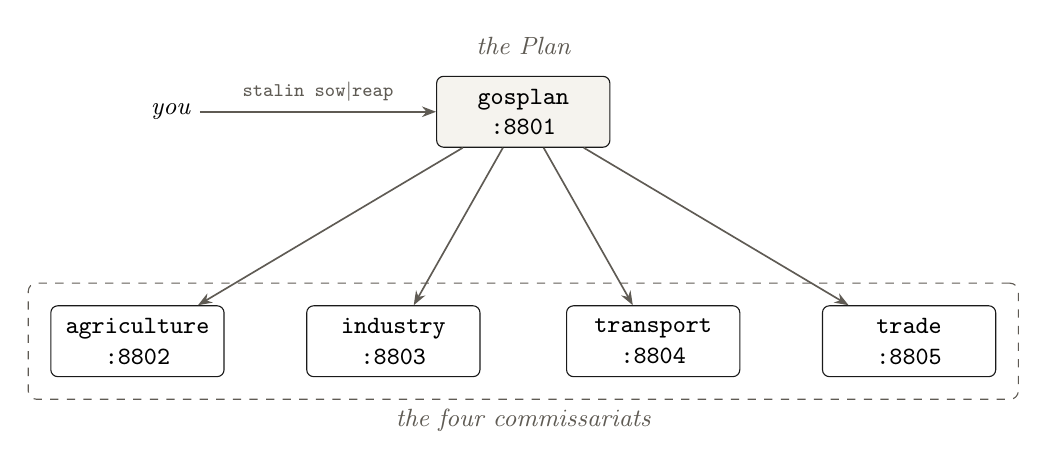
\begin{tikzpicture}[
  box/.style={draw=ink, fill=white, rounded corners=2.5pt, align=center,
              font=\small\ttfamily, inner sep=4.5pt, minimum width=22mm,
              minimum height=9mm},
]

\node[box, fill=pale, font=\small\ttfamily\bfseries] (gos) {gosplan\\:8801};
\node[lbl, above=1.5mm of gos, font=\small\itshape] {the Plan};
\node[font=\small\itshape] (you) [left=30mm of gos] {you};
\draw[ar] (you) -- node[above, pos=0.5, font=\scriptsize\ttfamily]{stalin sow$\mid$reap} (gos);

\node[box] (agri)  [below=20mm of gos, xshift=-49mm] {agriculture\\:8802};
\node[box] (ind)   [below=20mm of gos, xshift=-16.5mm] {industry\\:8803};
\node[box] (tran)  [below=20mm of gos, xshift= 16.5mm] {transport\\:8804};
\node[box] (trade) [below=20mm of gos, xshift= 49mm] {trade\\:8805};

\draw[ar] (gos) -- (agri);
\draw[ar] (gos) -- (ind);
\draw[ar] (gos) -- (tran);
\draw[ar] (gos) -- (trade);

\begin{scope}[on background layer]
\node[fit=(agri)(ind)(tran)(trade), draw=grey, dashed, rounded corners=3pt,
      inner sep=2.8mm, label={[subt, font=\small\itshape]below:the four commissariats}] {};
\end{scope}

\end{tikzpicture}
\end{center}

Every arrow is a delegation, and every arrow points away from the Plan. The Plan is the only
client any of them has. The four do not talk to each other.


\subsection{The game as a composite}

Each turn is one of the four compositions. Which one it is makes a claim about the year, rather
than being a detail of the code.

\begin{center}\small
\begin{tabular}{@{}llp{62mm}@{}}
\toprule
& \textbf{composite} & \textbf{why that one} \\
\midrule
spring & (agri $\boxtimes$ mill) $\boxtimes$ rail & all three work at once and \emph{all three
owe a report}. There is no partial year \\[1mm]
autumn & transport $\lhd$ trade & what may be sold is computed \emph{from} what the railway
actually moved \\[1mm]
build  & tractors $\times$ armaments & choose to invest in either tractors or armaments \\
\bottomrule
\end{tabular}
\end{center}

\subsection{What crosses, and what the status code says}

Every hop is a \texttt{POST} to a port with a JSON body, and the response is JSON. The port
identifies the container. The three outcomes are genuinely different kinds of
thing, and the status vocabulary already distinguishes them.

\begin{lstlisting}[language=TS]
try { body = await req.json(); }
catch { return json({ error: "not JSON" }, 400); }

const prompt = opts.parse(body);
if (prompt === null) {
  return json({ error: "not a valid prompt for this container", got: body }, 400);
}
try   { return json(await opts.answer(prompt, depth + 1), 200); }
catch (e) { return json({ error: msg }, 500); }
\end{lstlisting}


The depth rides in a header rather than in the prompt, because the prompt is the container's shape,
and nothing that isn't a prompt belongs in it.

\subsection{A hop is a CLI tool}

The program that carries a prompt to the next level is fifty lines long, and knows nothing about
the game. With the agriculture commissariat running, a single prompt can be fired at it by hand.

\begin{lstlisting}[language=SH]
$ deno run --quiet --allow-net --allow-env lib/delegate.ts 8802 \
    '{"tag":"Harvest","workforce":{"fields":100,"drivers":0,"mill":12,
      "rail":8,"dead":0},"tractors":0,"year":1928}' 0
{"grain":263.35,"grade":"adequate","perWorker":2.63,"withoutTractors":263.35}
\end{lstlisting}

That is the mapping $u$ made executable, and it observes every discipline from §\ref{sec:unix}.
Its exit codes distinguish the two kinds of failure. Exit code \texttt{2} for a malformed prompt or missing
arguments. Exit code \texttt{1} for a port with nothing behind it. Every diagnostic goes to descriptor~2, and
descriptor~1 carries the response and nothing else. That is exactly what lets the caller parse the
whole of stdout as one JSON document.

That discipline is also what makes the tracing possible. The servers narrate themselves on
descriptor~2 while descriptor~1 stays machine-readable.

\begin{lstlisting}[style=trace]
 ↓ gosplan   Sow order={"procurement":"firm","labour":{"…
   ↓ gosplan   ((agri (x) smelter) (x) transport)
     ↓ agri      Harvest workforce={"fields":96,"drivers":0,"mill":1… tractors=0 year=1928
     ↑ agri      {grain, grade, perWorker, withoutTractors}
     ↓ industry  Smelt workers=14 millCapacity=8 year=1928
     ↑ industry  {steel, idleCapacity}
     ↓ transport Lay workers=10 steel=10 year=1928
     ↑ transport {added, steelUsed}
 ↑ gosplan   {kind, year, harvest, steel, …}
\end{lstlisting}

Indentation is the depth counter. The arrow \texttt{↓} is control flowing down. The arrow
\texttt{↑} is data flowing back up. The tracer prints at most thirty-four characters of any value
and then gives up, which is what the \texttt{…} is.

The second line is the one to look at. It is a runner's \texttt{label}, and labels compose. A
pass-through runner is given one when it is built. Every combinator makes its own out of the labels of its parts, in the
algebra's own notation.

\begin{lstlisting}[language=TS]
label: `(${a.label} (x) ${b.label})`    // the tensor
label: `(${a.label} x ${b.label})`      // the product
label: `(${a.label} <| ${b.label})`     // the sequential
label: `(${a.label} + ${b.label})`      // the sum
\end{lstlisting}

So \texttt{((agri (x) smelter) (x) transport)} is not a comment anybody wrote. It is the expression
that built that runner, printing itself, and the four hops indented beneath it are what the
expression turned into. That is a derivation tree of container morphisms, printed by a program that
had no idea it was doing that.

\subsection{Where the compiler carries a rule of the game}

Two rules are enforced by the type checker rather than validated at run time. Both work by the
trick from \S\ref{sec:cond}, a conditional type over a finite union.

\begin{lstlisting}[language=TS]
export type ExportChoice<G extends HarvestGrade> =
  G extends "failure"  ? "none"
: G extends "poor"     ? "none" | "surplus"
: G extends "adequate" ? "none" | "surplus" | "full"
:                        "none" | "surplus" | "full" | "maximum";

exportPlan("bumper",  "maximum")   // fine
exportPlan("failure", "maximum")   // does not compile
\end{lstlisting}

Exporting grain during a failed harvest is not a move the engine rejects. It is a move that
cannot be written down. The same trick carries the arc of the whole game. You may buy steel while
in deficit, and never sell it. A country that exports its steel is not industrialising.

\begin{lstlisting}[language=TS]
export type SteelTrade<P extends SteelPosition> =
  P extends "deficit" ? "none" | "buy" : "none";
\end{lstlisting}

Both work only because the index set is finite. A rule over tonnages could not be typed this way.
The same rule over \emph{grades} can. That is also how the apparatus actually worked. Quotas were
set against reported categories, never against measured tonnes.

\subsection{The one thing that cannot cross}

Of everything JSON leaves out, one omission bites structurally rather than merely requiring care.
A function cannot be serialised. And the shape of $\lhd$ is a first prompt together with a function
computing the second.

So sequential composition cannot be distributed over the wire. It is resolved \emph{above} it, in
the runner. The runner prompts the first container, then applies that function to the response to
obtain the second prompt. Only the two ground prompts ever cross.

The wire format is not neutral about which combinators can be sent and which must be interpreted
locally. This is the sharpest example in the repository of a mathematical structure meeting a
transport and losing an argument.

\subsection{What the reports are worth}

Each commissariat holds two things the Plan cannot see. How well it is actually doing. And how
much it inflates its dispatches. The Plan keeps the true ledger for grain, because the grain
physically exists. What diverges is the \emph{report}. And you plan against the report.

\begin{lstlisting}
Narkomtiazhprom: quota fulfilled, with difficulties overcome.
\end{lstlisting}

This is the honest limit of everything above. The type of a dispatch guarantees its shape and says
exactly nothing about its truth. A validator can establish that a response is a well-formed dispatch.
No validator can establish that the number in it is the number that happened. The reckoning prints
both columns and leaves the reader to notice.

\subsection{And where the protocol is not doing the work}

One last piece of honesty. HTTP is stateless and these servers are not. Each keeps its books at
module scope, in the process. That is defensible. A commissariat \emph{is} a stateful thing, and
the exercise is about the container algebra rather than about session management. But it has a
consequence, and the consequence is visible in the interface. The protocol cannot clear that state.
So clearing it has to become a prompt.

\begin{lstlisting}[language=TS]
Reset: (p) => { seed = p.seed; books = new Books(...); laid = 0; lastQuota = 0;
                return { ok: true }; },
\end{lstlisting}

The prompt \texttt{Reset} has no meaning in the fiction. No plan resets a railway. It exists because starting
a new game must reach the commissariats. Otherwise the weather and the books carry over into the
next one, and the comment records that as a bug that actually happened. Determinism on the seed is
what makes a playthrough a regression test, so this is load-bearing rather than tidying. And the
general lesson is the one worth taking away. When process state substitutes for protocol state, the
lifecycle leaks into the interface.

\newpage

\section*{Conclusion}

\begin{sectionbox}
What has been built is a \emph{fake}. Containers for event-driven programming, faked with CLI
tools and TypeScript \texttt{async} event handlers.

The nicest thing about this fake is that you can substitute \texttt{claude} for any of the CLI
tools.
\end{sectionbox}

The impersonation has three parts.

A container $(P, R)$ becomes a tagged union together with a lookup indexed by its tags. That works,
and works only, because the tag set is \emph{finite}. Over a finite index a dependent type is just
a table, and a table is something TypeScript can write down.

The inhabitant $(p : P) \to R\,p$ becomes the handler record. The compiler enforces its totality,
because it is a mapped type over that same union.

And a morphism becomes an \texttt{async} function. That is where the two directions meet.

\begin{lstlisting}[language=TS]
const reply = await lower.run(u(prompt));   // the prompt, going down
return f(prompt, reply);                    // the reply, coming back
\end{lstlisting}

\subsection{The response flows backwards}

That is the part worth dwelling on. Control flows \emph{down}. A handler is woken by a prompt. It
computes a lower-level prompt with $u$, and fires it. In this implementation that means spawning a
process and opening a socket, so the descent is a real one, made of real programs. Then it stops.
At the \texttt{await} the handler suspends and hands the runtime back. The runtime is free to wake
other handlers while it waits.

The response then flows \emph{backwards} along the path the prompt took. Each response resumes the
handler that fired the prompt, at the very line it stopped on. That handler applies $f$ to turn the
response into its own. So $u$ runs on the way down and $f$ on the way back up, in one function body,
read top to bottom, with the suspension between them invisible in the text.

And where the fake fails, it fails visibly. Sequential composition cannot be sent over the wire,
because its shape contains a function and functions do not serialise. A validated response is
guaranteed to have the right shape, and is guaranteed nothing about its truth. Both limits are
consequences of the same substrate that made the impersonation possible in the first place. That is
the honest summary of the whole exercise. The algebra is real, and everything holding it up is
Unix.

\end{document}


